\documentclass[conference]{IEEEtran}
\IEEEoverridecommandlockouts
\usepackage{cite}
\usepackage{amsmath,amssymb}
\usepackage{graphicx}
\usepackage{booktabs}
\usepackage{xcolor}
\usepackage{url}
\usepackage[hidelinks]{hyperref}
\graphicspath{{../docs/figures/}}
\makeatletter
\newcommand{\linebreakand}{%
  \end{@IEEEauthorhalign}\hfill\mbox{}\par
  \mbox{}\hfill\begin{@IEEEauthorhalign}}
\makeatother

\begin{document}

\title{Instruction and Data Memory Hierarchy:\\
Harvard, Modified-Harvard and Shared-Memory\\
Organisations in Verilog\\
{\large Final (Phase II) Report -- Modern Computer Architecture, Project 9}}

\author{
\IEEEauthorblockN{Aaryan Yadav}
\IEEEauthorblockA{2401010011}
\and
\IEEEauthorblockN{Shashwat Sinha}
\IEEEauthorblockA{2401010438}
\and
\IEEEauthorblockN{Shivam Mishra}
\IEEEauthorblockA{2401010442}
\and
\IEEEauthorblockN{Himank Kaushik}
\IEEEauthorblockA{2401010187}
\and
\IEEEauthorblockN{Satyam Kumar}
\IEEEauthorblockA{2401010429}
\linebreakand
\IEEEauthorblockA{\textit{B.Tech CSE (AI), Rishihood University, Sonipat, Haryana, India}}
}

\maketitle

% ---------------------------------------------------------------------------
\begin{abstract}
A processor fetches instructions and reads and writes data. If both kinds of
access share one memory port (Von Neumann), a load or store must wait for the
instruction fetch---a structural hazard. Giving them separate paths (Harvard)
removes the conflict. This project implements both organisations in
synthesisable Verilog around one unchanged single-cycle RV32I-subset core.
Phase~I built a Harvard system (program counter, 4\,KB instruction memory,
4\,KB data memory, address decoder, read/write control, memory-mapped I/O) and
a Von Neumann baseline; Harvard ran every program at CPI\,=\,1.00 against
1.02--1.31 for the baseline. Phase~II adds the optional \emph{shared
lower-level memory}: an 8\,KB main memory with configurable latency that holds
both code and data, reached through either split level-1 instruction and data
caches with a 2-client arbiter (modified Harvard, proposed) or one unified
single-ported L1 cache of the same total size (Von Neumann hierarchy). All
designs are verified by a self-checking testbench against a Python golden
instruction-set simulator, and every cache counter matches an independent cache
model exactly: 274 simulation runs and 20 directed unit checks pass. With an
8-cycle main memory and 512\,B of L1, the split hierarchy has a geometric-mean
CPI of 2.01 against 2.81 for the unified cache and 12.3 without caches, a
$1.40\times$ and $6.1\times$ speed-up; its read miss rate is 4.0\,\% against
8.9\,\% and its average memory access time 1.64 against 2.15 cycles. Yosys
synthesis shows that the split hierarchy uses about 5\,\% fewer LUTs than the
unified one.
\end{abstract}

\begin{IEEEkeywords}
Harvard architecture, Von Neumann architecture, memory hierarchy, cache,
modified Harvard, AMAT, address decoding, RISC-V, Verilog
\end{IEEEkeywords}

% ---------------------------------------------------------------------------
\section{Introduction}
Every instruction must be \emph{fetched}, and about a quarter to a third of
instructions also \emph{load or store} data. How the memory is organised
decides whether these accesses overlap or take turns, and therefore sets the
cycles per instruction (CPI) of a simple processor.

The project brief \cite{mca_projects} asks us to ``implement a simplified
Harvard-style memory organisation with separate instruction and data paths and
analyse its behaviour'', suggesting a program counter, instruction memory, data
memory, address decoder, read/write control and an \emph{optional shared
lower-level memory}, and asks for the RTL, a block diagram, simulation
waveforms and a comparison with a shared-memory organisation. Phase~I
delivered the Harvard design and the comparison for ideal single-cycle
memories. Phase~II asks what happens in a realistic system where the memory
behind the processor is slow and \emph{shared}: we add a lower-level memory
with configurable latency and compare four organisations built from the same
core and the same main memory:
\begin{enumerate}
\item \textbf{VN-flat}: one port, no cache (classic Von Neumann bottleneck);
\item \textbf{Split-flat}: split I/D ports, no cache, shared slow memory;
\item \textbf{Unified L1}: one single-ported 512\,B cache for code and data;
\item \textbf{Split L1} (proposed): 256\,B I-cache + 256\,B D-cache sharing
the main memory through an arbiter---a \emph{modified Harvard} hierarchy.
\end{enumerate}

% ---------------------------------------------------------------------------
\section{Literature Review}

\subsection{Origins of the two organisations}
The stored-program design described by von Neumann in the EDVAC report
\cite{vonneumann1945} keeps instructions and data in one memory: programs are
just data, and one memory is cheap. The Harvard Mark~I \cite{aiken1946} read
instructions from paper tape and kept data in separate counters, giving the
name ``Harvard architecture'' to machines with separate instruction and data
storage.

\subsection{The Von Neumann bottleneck and the memory wall}
Backus \cite{backus1978} called the single processor--memory channel the
``von Neumann bottleneck''. Wulf and McKee \cite{wulf1995} showed that, as
processors outpaced DRAM, average memory access time would dominate
performance (the ``memory wall''). Both arguments call for more memory
bandwidth close to the processor and for hiding the latency of the slow
memory behind it.

\subsection{Split memories and caches}
Textbook RISC datapaths \cite{patterson2020,harris2021} use separate
instruction and data memories so that a single-cycle or pipelined core can
fetch and load/store in the same cycle; with one memory, the MEM stage of one
instruction collides with the IF stage of another and a stall is needed
\cite{hennessy2017}. Real machines are \emph{modified Harvard}: split L1
instruction and data caches backed by a unified lower level so that software
still sees one address space \cite{smith1982,hennessy2017}. Smith's survey
\cite{smith1982} discusses the split-versus-unified choice: a split cache
doubles bandwidth and lets each half be tuned, while a unified cache can share
its capacity flexibly between code and data. Hill and Smith
\cite{hill1989} classify misses as compulsory, capacity and conflict (the
``three Cs''); direct-mapped caches are fast and simple but suffer conflict
misses. Jouppi \cite{jouppi1993} showed that write-through caches with small
write buffers hide most store latency. Microcontrollers such as the ARM
Cortex-M3 expose separate ICode, DCode and System buses \cite{arm_m3}, while
area-optimised cores such as PicoRV32 \cite{picorv32} use one unified memory
interface and accept extra cycles per memory instruction.

\subsection{Gap addressed by this project}
Course designs usually show the Harvard datapath only inside a full CPU and
rarely quantify what the split buys, especially once a slow shared memory is
involved. We provide a \emph{controlled} comparison: identical core RTL,
programs, address map and main memory, with only the memory organisation
changed, measured by hardware performance counters and cross-checked against
an independent golden model.

% ---------------------------------------------------------------------------
\section{Proposed Solution}

\subsection{Processor core and address map}
The core (\texttt{cpu\_core.v}) is a single-cycle RV32I subset
\cite{riscv_isa}: ADD, SUB, AND, OR, XOR, SLT, SLL, SRL, their immediate
forms, LW, SW, BEQ, BNE, BLT, BGE, JAL, JALR and LUI. It is
\emph{memory-organisation agnostic}: it exposes an instruction port
(PC\,$\rightarrow$\,instruction), a data port (address, write data, strobes
\,$\rightarrow$\,read data) and a \texttt{stall} input that freezes the PC and
all architectural writes. Phase~II added one output, \texttt{d\_wreq}, the
store request before stall gating, so that a cache can decide to stall
without creating a combinational loop. All designs share the address map in
Table~\ref{tab:map}.

\begin{table}[h]
\caption{Common address map}
\label{tab:map}
\centering
\begin{tabular}{lll}
\toprule
Range & Device & Access \\
\midrule
\texttt{0x0000\_0000--0FFF} & Instruction region (4\,KB) & fetch \\
\texttt{0x0000\_1000--1FFF} & Data region (4\,KB) & load/store \\
\texttt{0x0000\_2000/04/08} & I/O: OUT, HALT, CYCLE & st/st/ld \\
other & -- & bus error \\
\bottomrule
\end{tabular}
\end{table}

\subsection{Phase I: Harvard organisation and baseline}
\texttt{harvard\_top.v} (Fig.~\ref{fig:harvard}) connects the instruction port
to a 1024-word instruction ROM (\texttt{imem.v}, asynchronous read) and the
data port to an \textbf{address decoder} (\texttt{addr\_decoder.v}), which
turns the upper address bits into one-hot selects for data memory or I/O and
flags a bus error for unmapped addresses, including data accesses to the
instruction region. A \textbf{read/write control} unit
(\texttt{rw\_control.v}) sends the strobes only to the selected device and
multiplexes its read data back. The \textbf{data memory} (\texttt{dmem.v}) is
a 1024-word RAM. \texttt{vonneumann\_top.v} connects the \emph{same} core to
one single-ported 8\,KB memory through a two-state FETCH/DATA arbiter: a
fetched load/store is latched into an instruction register and executed in an
extra DATA cycle, so
\begin{equation}
\text{CPI}_{\text{H}} = 1, \qquad \text{CPI}_{\text{VN}} = 1 + f_{\text{mem}},
\label{eq:model}
\end{equation}
where $f_{\text{mem}}$ is the fraction of instructions that are loads or stores.

\begin{figure}[t]
\centering
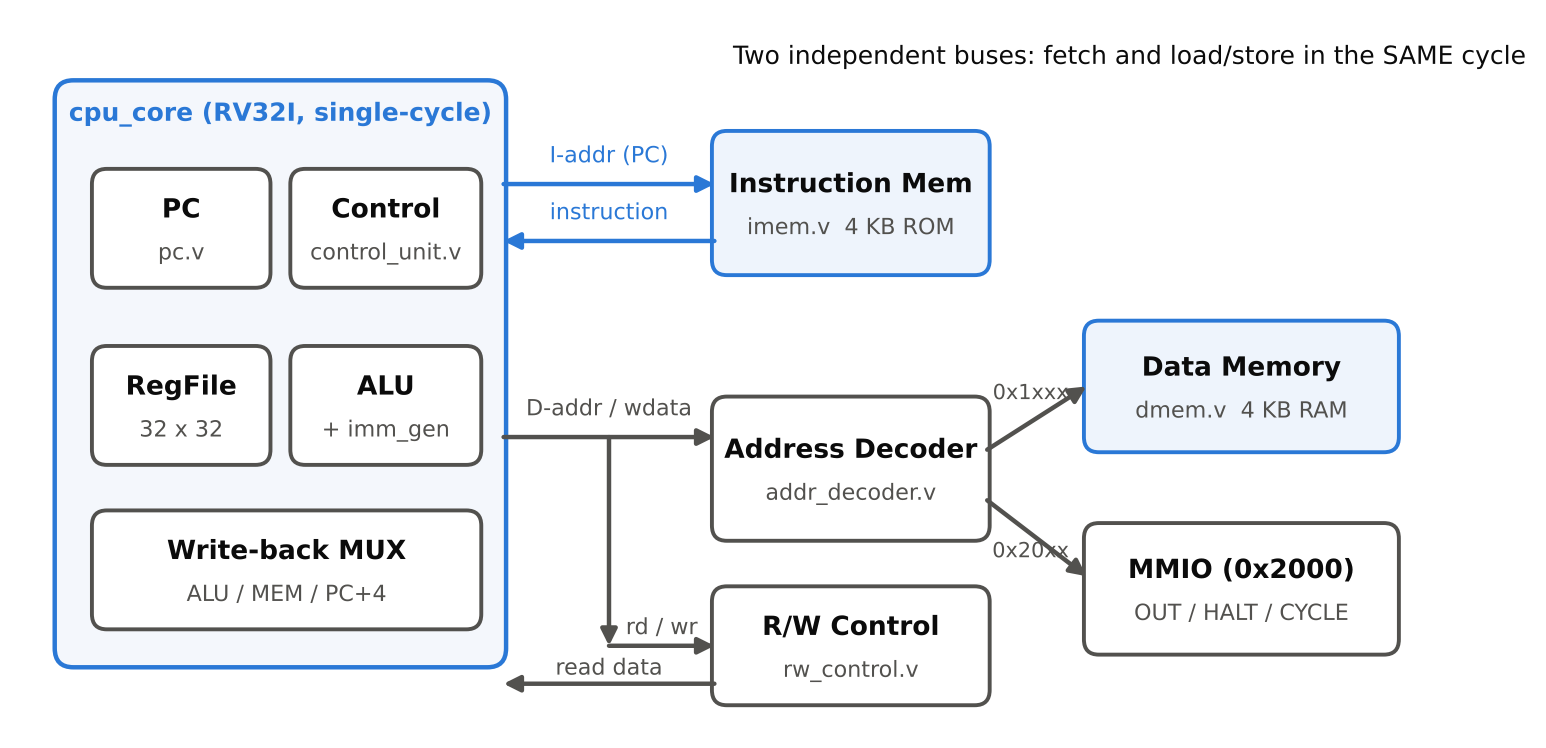
\includegraphics[width=\columnwidth]{block_harvard.png}
\caption{Phase I Harvard organisation: separate instruction and data buses.}
\label{fig:harvard}
\end{figure}

\subsection{Phase II: shared lower-level memory}
\texttt{main\_mem.v} is one single-ported 8\,KB memory holding both code
(words 0--1023) and data (words 1024--2047). A request accepted in cycle $t$
returns its first word in cycle $t+\text{LAT}$ and then one word per cycle, so
a cache line of $W$ words is a burst. Writes complete after LAT cycles.
LAT is a parameter (1--16 cycles in our sweeps).

\subsection{Phase II: L1 cache}
\texttt{l1\_cache.v} is one parameterised, direct-mapped cache used as the
instruction cache, the data cache and the unified cache:
\begin{itemize}
\item \textbf{Hit path:} tag compare and data read are combinational, so a hit
adds no cycles to the single-cycle core.
\item \textbf{Read miss:} the core is stalled while the whole line is fetched
as one burst; the miss penalty is $\text{LAT}+W$ cycles.
\item \textbf{Writes:} write-through, no-write-allocate, through a one-entry
\emph{write buffer}. A store completes in one cycle if the buffer is empty and
drains to memory in the background \cite{jouppi1993}. A read miss waits until
the buffer has drained, so a load can never read stale memory.
\item \textbf{Storage:} the data and tag arrays each have one write port and
no reset, so synthesis maps them to distributed RAM (an early version with two
write ports produced 2\,k flip-flops per cache).
\item \textbf{NOCACHE mode:} one line of one word that is invalidated after
each use, giving the ``flat'' no-cache baselines from the same RTL.
\end{itemize}

\subsection{Proposed modified-Harvard hierarchy}
\texttt{modharvard\_top.v} (Fig.~\ref{fig:hier}a) gives the core a private
I-cache on the instruction port and, behind the Phase~I decoder and read/write
control, a private D-cache on the data port. I/O stays uncached and acts as a
fence: an I/O access waits for the write buffer, so the HALT store is ordered
after every earlier store. The two caches meet only at \texttt{mem\_arbiter.v},
which grants the idle main memory to one requester, latches the owner to route
the burst back, and flags a \emph{conflict} in any cycle where both caches
request. The I-side has priority because an instruction miss always stalls
the core, while a write-buffer drain usually does not. While the I-cache
misses, the placeholder instruction is a NOP and all data-side requests are
masked, so no spurious data access can occur.

\subsection{Von Neumann hierarchy baseline}
\texttt{unicache\_top.v} (Fig.~\ref{fig:hier}b) keeps the Phase~I FETCH/DATA
arbiter, but its single port now leads to one unified 512\,B L1 cache (same
total capacity as the split pair) in front of the same main memory. A
load/store therefore still costs a structural-hazard cycle, and code and data
now compete for the same cache lines.

\begin{figure}[t]
\centering
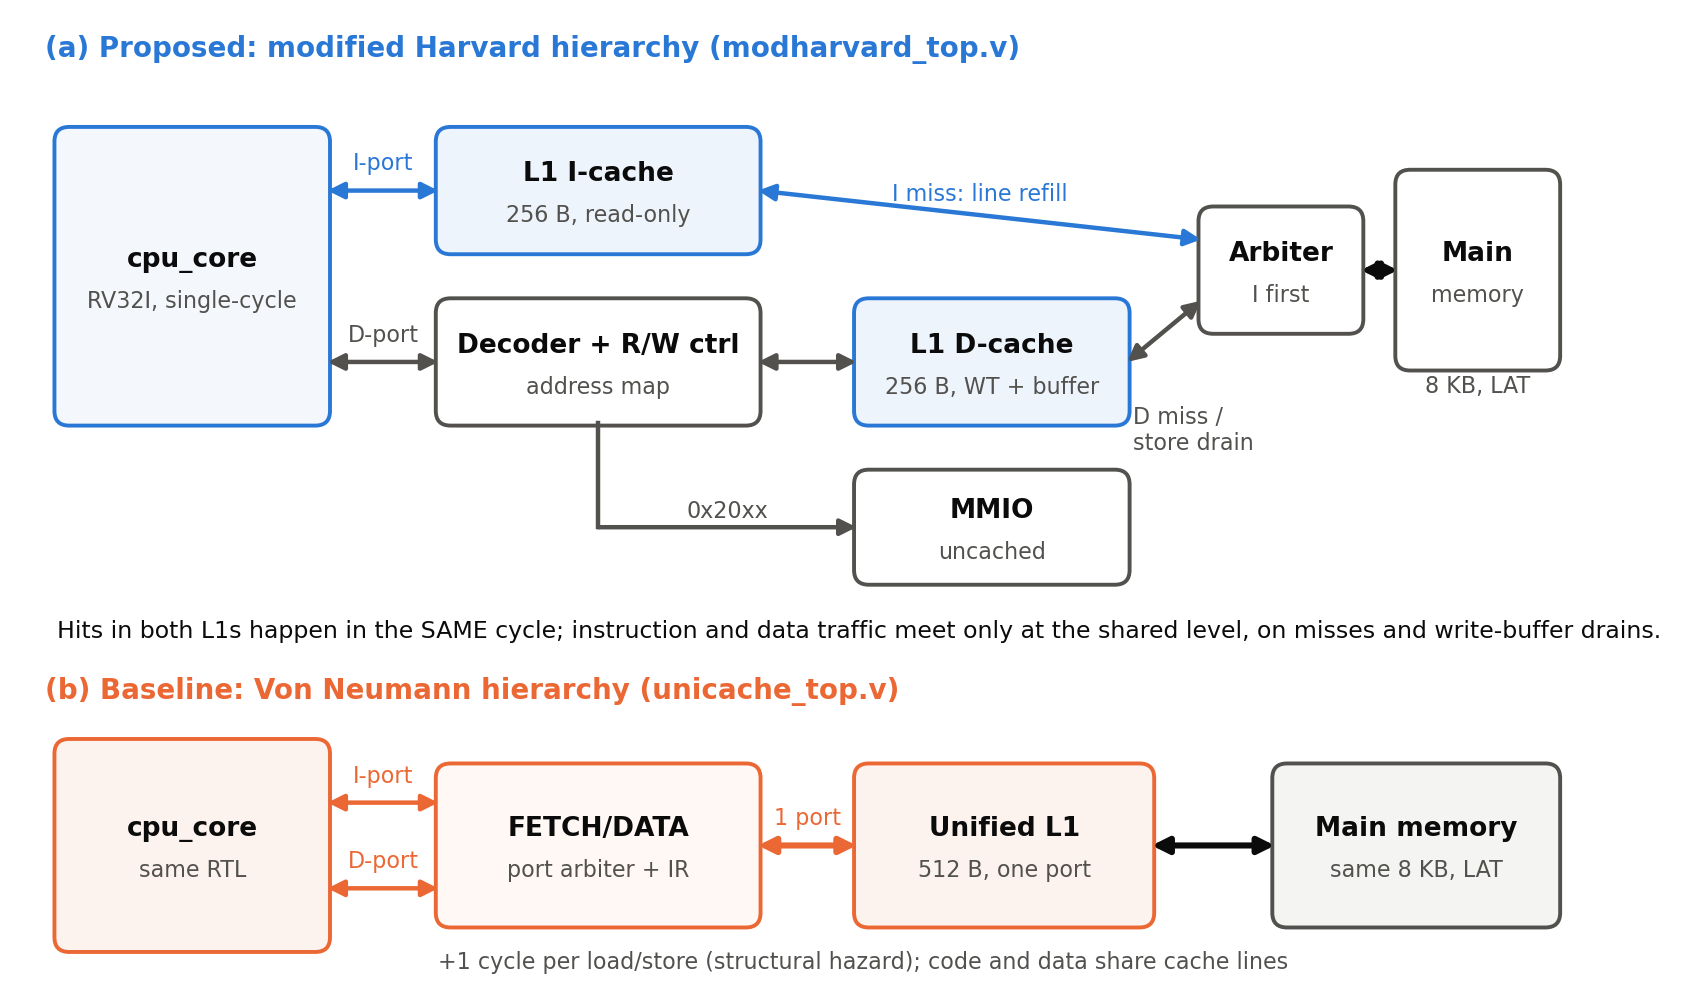
\includegraphics[width=\columnwidth]{block_hierarchy.png}
\caption{Phase II: (a) proposed split-L1 hierarchy over a shared main memory;
(b) unified-L1 baseline with the same capacity and memory.}
\label{fig:hier}
\end{figure}

\subsection{Verification methodology}
A two-pass assembler and instruction-set simulator in Python
(\texttt{sw/rv32\_asm.py}) produces, for each program, the code and data
images, the \emph{expected} final data image, cycle predictions for
(\ref{eq:model}) and, new in Phase~II, the ordered trace of every fetch, load
and store. \texttt{sw/cache\_model.py} replays that trace through a software
model of the caches. Because the caches are direct-mapped and never allocate
on a write, the hit/miss sequence depends only on access order, not on timing,
so the hardware counters must match the model \emph{exactly}. Each
hierarchy run (\texttt{tb/tb\_hier.v}, \texttt{sim/run\_hier.py}) passes only
if (i) the final data region of main memory equals the golden image, (ii) the
write buffer is empty at HALT, (iii) the I/D read, miss, write and write-hit
counts equal the model, and (iv) the cycle accounting closes:
\begin{equation}
\text{cycles} = \text{instret} + \sum \text{stall}_{\text{imiss, dmiss, wbuf, io, struct}}.
\end{equation}
Two directed unit testbenches cover the address decoder (9 checks) and the
cache with main memory (11 checks: cold-miss penalty of exactly
$\text{LAT}+W$ cycles, same-line hit, store hit in one cycle, back-to-back
store waiting $\text{LAT}+1$ cycles, conflict eviction, load-after-buffered-store
correctness, and write-through contents). Seven programs are used:
\texttt{fibonacci}, \texttt{array\_sum}, \texttt{vector\_add},
\texttt{bubble\_sort} (Phase~I) and, new in Phase~II, \texttt{matmul} (4$\times$4
matrix product with a shift-and-add multiply subroutine, 2\,596 instructions),
\texttt{memcpy} (64-word streaming copy) and \texttt{unrolled\_sum} (a 512\,B
unrolled loop body chosen to overflow a 256\,B I-cache). Simulation uses Icarus
Verilog \cite{icarus}; synthesis uses Yosys \cite{yosys}.

% ---------------------------------------------------------------------------
\section{Results and Discussion}

\subsection{Ideal memories (Phase I)}
With single-cycle memories every Harvard run completes at CPI\,=\,1.00, and the
baseline matches (\ref{eq:model}) exactly (Table~\ref{tab:p1}). The Harvard
counters report as many \emph{parallel} cycles (fetch and data access in the
same clock) as the baseline has stall cycles, e.g.\ 49 for
\texttt{vector\_add} (Fig.~\ref{fig:waves}).

\begin{table}[h]
\caption{Phase I: ideal single-cycle memories}
\label{tab:p1}
\centering
\setlength{\tabcolsep}{4pt}
\begin{tabular}{lrrrrr}
\toprule
Program & Instr. & $f_{\text{mem}}$ & H cyc. & VN cyc. & Speed-up \\
\midrule
fibonacci   & 128 & 1.6\%  & 128 & 130 & 1.02$\times$ \\
array\_sum  & 176 & 19.9\% & 176 & 211 & 1.20$\times$ \\
bubble\_sort& 633 & 31.1\% & 633 & 830 & 1.31$\times$ \\
vector\_add & 156 & 31.4\% & 156 & 205 & 1.31$\times$ \\
\bottomrule
\end{tabular}
\end{table}

\begin{figure*}[t]
\centering
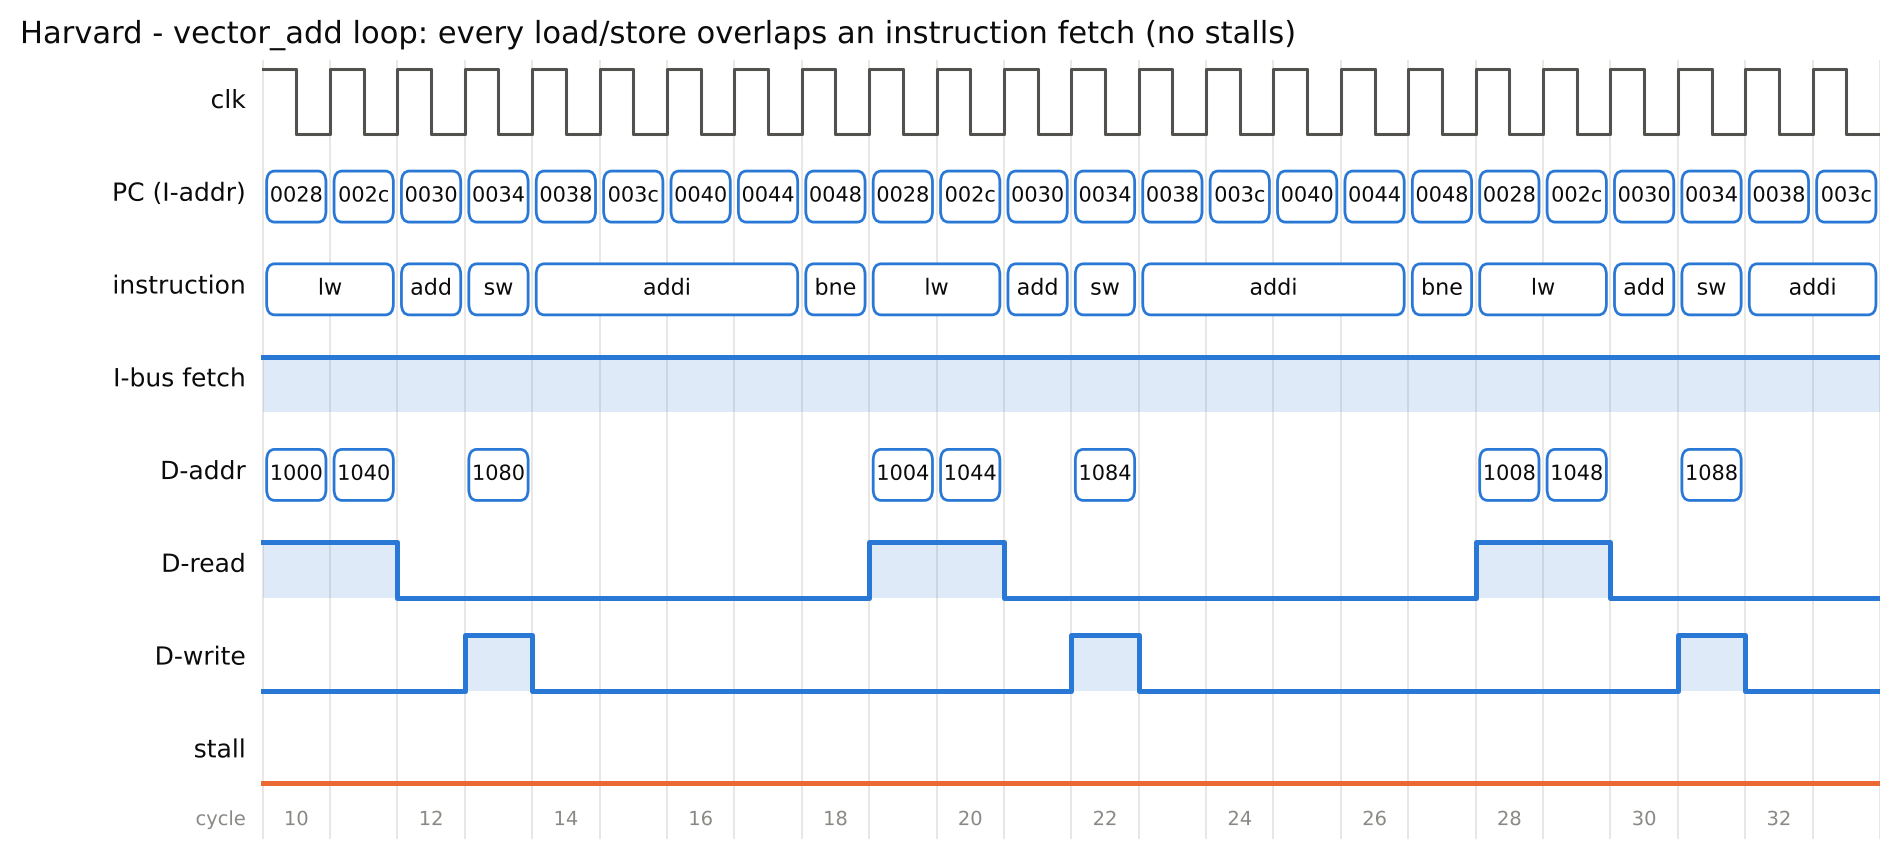
\includegraphics[width=0.49\textwidth]{wave_harvard.png}\hfill
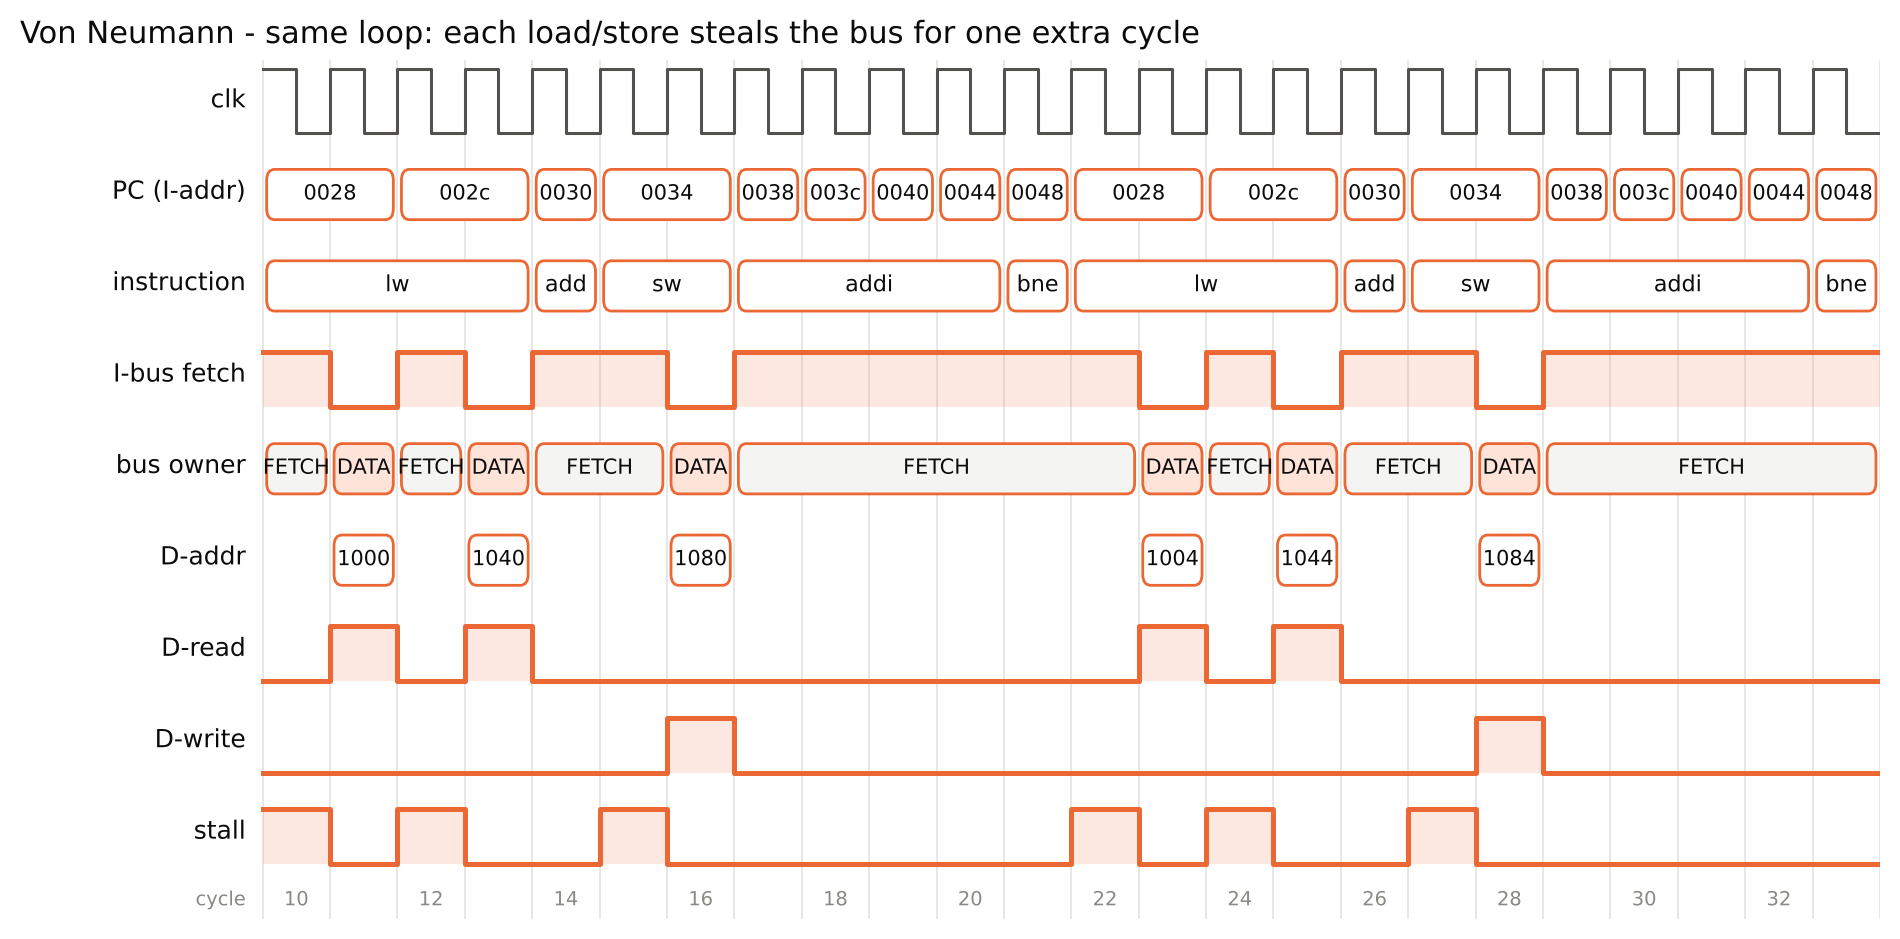
\includegraphics[width=0.49\textwidth]{wave_vonneumann.png}
\caption{Phase I waveforms, \texttt{vector\_add}: Harvard (left) overlaps fetch
with every load/store; Von Neumann (right) adds a DATA cycle for each.}
\label{fig:waves}
\end{figure*}

\subsection{Effect of main-memory latency}
Fig.~\ref{fig:lat} shows the geometric-mean CPI of the seven programs as the
main-memory latency grows. Without caches both flat designs scale almost
linearly with latency (CPI 12.3 and 12.0 at $\text{LAT}=8$, about 22 at 16)
because every instruction pays a memory access. Splitting the ports without
caches buys only 2--8\,\% (geo-mean, from $\text{LAT}=16$ down to 1): the single slow memory is still shared, so the
Harvard advantage disappears whenever the lower level is the bottleneck. Adding
caches changes the picture: at $\text{LAT}=8$ the unified L1 reaches CPI 2.81
and the split L1 2.01, and the gap \emph{widens} with latency (CPI 4.05 vs
2.85 at $\text{LAT}=16$), because the split design misses less and each miss
costs more.

\begin{figure}[t]
\centering
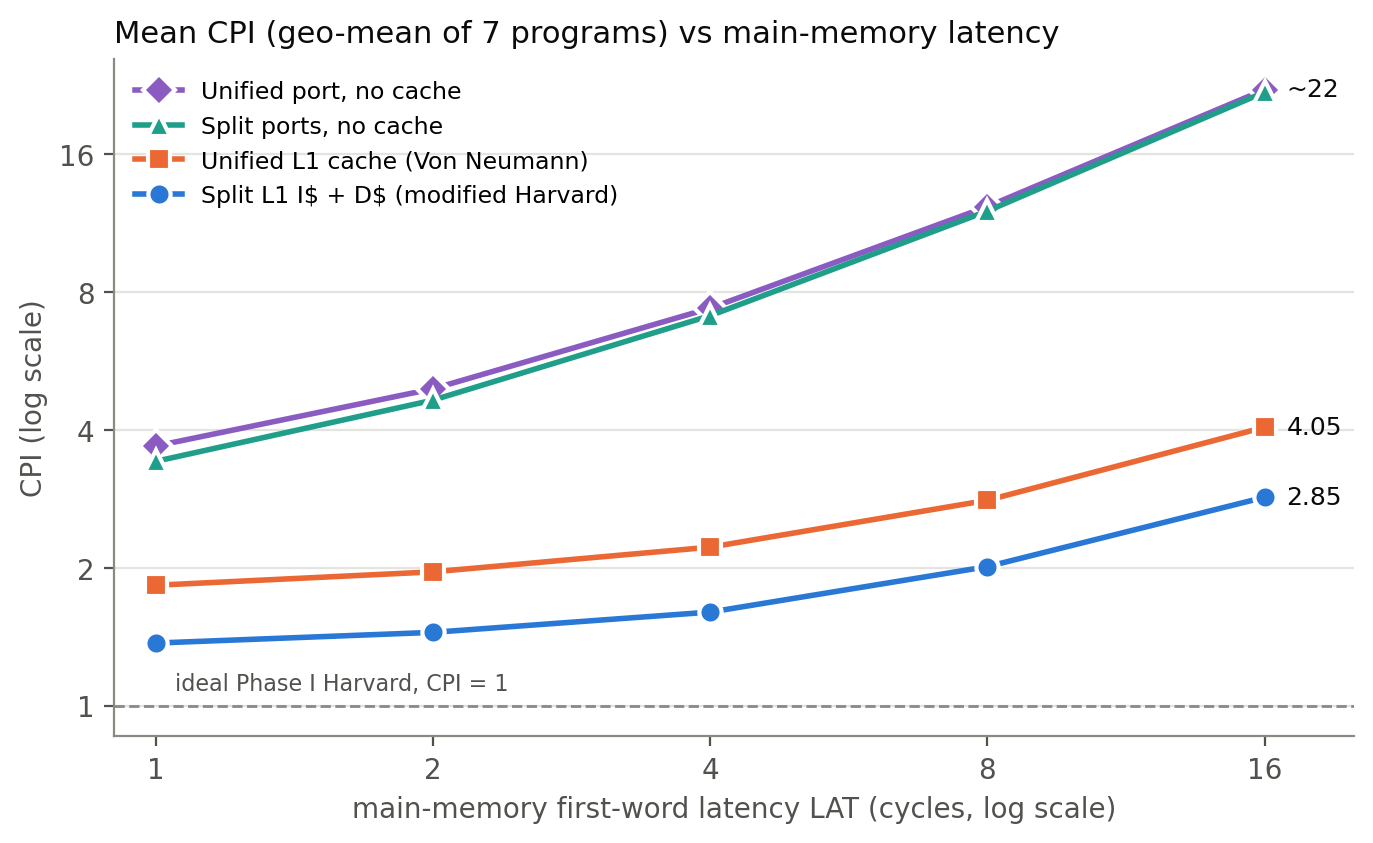
\includegraphics[width=\columnwidth]{cpi_vs_latency.png}
\caption{Mean CPI vs main-memory latency (L1: 2$\times$256\,B split or 512\,B
unified, 16\,B lines).}
\label{fig:lat}
\end{figure}

\begin{table}[t]
\caption{Phase II cycles, $\text{LAT}=8$, 512\,B of L1, 16\,B lines}
\label{tab:p2}
\centering
\setlength{\tabcolsep}{3pt}
\begin{tabular}{lrrrrrr}
\toprule
Program & Instr. & VN-flat & Split-flat & Unified & Split & $S_{\text{U}}$ \\
\midrule
array\_sum    & 176  & 2\,092  & 2\,056  & 556   & 351   & 1.58$\times$ \\
bubble\_sort  & 633  & 8\,291  & 8\,062  & 1\,689 & 1\,080 & 1.56$\times$ \\
fibonacci     & 128  & 1\,291  & 1\,288  & 199   & 196   & 1.02$\times$ \\
matmul        & 2\,596 & 27\,401 & 27\,240 & 4\,614 & 2\,872 & 1.61$\times$ \\
memcpy        & 394  & 5\,221  & 5\,028  & 1\,119 & 908   & 1.23$\times$ \\
unrolled\_sum & 549  & 8\,061  & 7\,802  & 2\,662 & 2\,405 & 1.11$\times$ \\
vector\_add   & 156  & 2\,041  & 1\,976  & 668   & 357   & 1.87$\times$ \\
\midrule
\multicolumn{2}{l}{geo-mean CPI} & 12.28 & 12.01 & 2.81 & 2.01 & 1.40$\times$ \\
\bottomrule
\end{tabular}
\\[2pt]\footnotesize $S_{\text{U}}$ = speed-up of split L1 over unified L1.
Split vs VN-flat: 3.35--9.54$\times$ (geo-mean 6.11$\times$).
\end{table}

\subsection{Where the cycles go}
Table~\ref{tab:p2} lists the cycle counts at $\text{LAT}=8$ and
Fig.~\ref{fig:stall} splits the CPI by cause. The split hierarchy beats the
unified cache on every program, for three reasons:
\begin{enumerate}
\item \textbf{No port conflict.} Each load/store in the unified design costs
one structural cycle (orange). The split design serves an I-hit and a D-hit in
the \emph{same} cycle: its \emph{parallel} counter equals the unified design's
structural-stall count minus the final uncached HALT store (48 vs 49 for
\texttt{vector\_add}, 144 vs 145 for \texttt{matmul}). The Phase~I advantage
survives inside the hierarchy.
\item \textbf{No code/data interference.} The code region starts at
\texttt{0x0000} and the data region at \texttt{0x1000}; since 4\,KB is a
multiple of the cache size, the first code lines and the first data lines map
to the \emph{same sets} of the direct-mapped unified cache and keep evicting
each other. For \texttt{matmul} the D-miss rate is 55\,\% in the unified cache
against 6\,\% in the split D-cache; the I-miss rate is 3.2\,\% vs 0.5\,\%.
\item \textbf{Little traffic at the shared level.} Across all programs the
arbiter sees both caches requesting in the same cycle at most once per run:
once the L1s filter the traffic, the shared lower level is rarely a
bottleneck. The geo-mean read miss rate is 4.0\,\% (split) against 8.9\,\%
(unified), giving an average read access time
$\text{AMAT} = 1 + m\,(\text{LAT}+W)$ of 1.64 vs 2.15 cycles.
\end{enumerate}

\begin{figure*}[t]
\centering
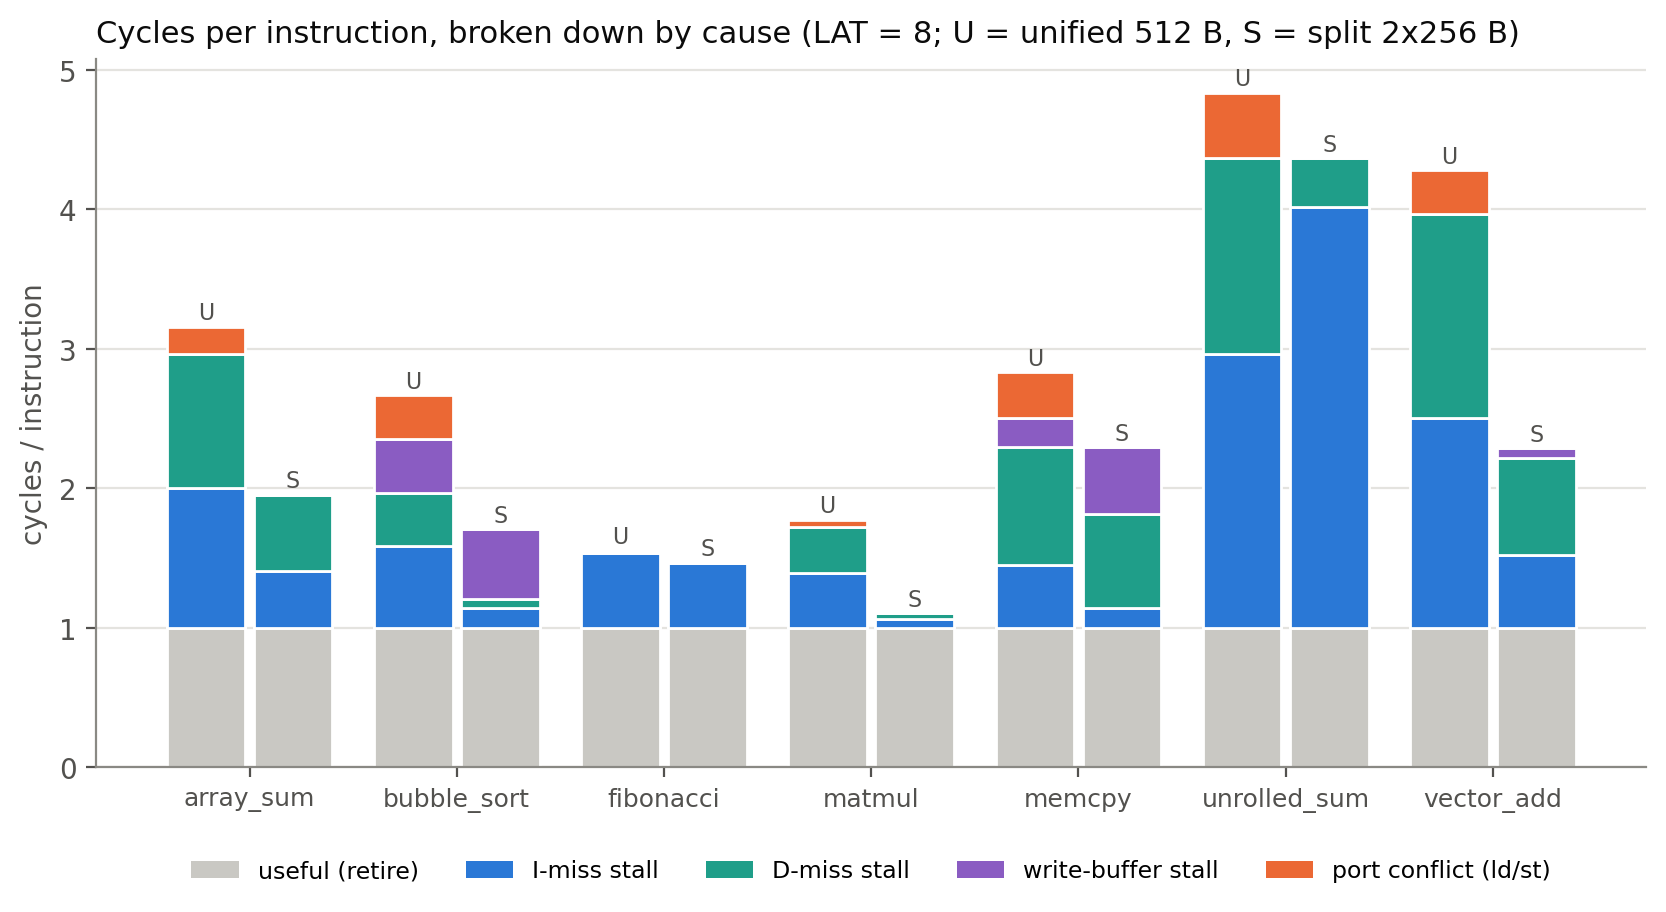
\includegraphics[width=0.8\textwidth]{stall_breakdown.png}
\caption{CPI by cause at $\text{LAT}=8$. U: unified 512\,B; S: split
2$\times$256\,B. Grey is the one useful cycle per instruction.}
\label{fig:stall}
\end{figure*}

The breakdown also shows where the split design is weaker.
\texttt{unrolled\_sum} has a 512\,B unrolled loop body that does not fit a 256\,B I-cache;
the unified cache can give more of its 512\,B to code, so its I-miss rate is
lower (16\,\% vs 25\,\%). A fixed split of capacity is the known cost of a
split cache \cite{smith1982}, yet the split design still wins by 1.11$\times$
because the unified design pays structural cycles and D-misses. Stores
expose the one-entry write buffer: in \texttt{bubble\_sort} and
\texttt{memcpy} a second store arriving before the first has drained waits
$\text{LAT}+1$ cycles (purple). A deeper buffer would remove most of this.
\texttt{fibonacci} keeps its data in registers, so the two designs are
almost equal (1.02$\times$), which is consistent with Phase~I.

\subsection{Cache size and line size}
Fig.~\ref{fig:size} varies the total L1 capacity at $\text{LAT}=8$. The split
design has the lower miss rate and CPI at every size; the unified cache
flattens at about 8.8\,\% misses and CPI 2.78 because its structural cycles
and code/data conflicts do not shrink with more capacity. Fig.~\ref{fig:line}
varies the line size at a fixed 512\,B. Longer lines exploit spatial locality
and lower the split design's CPI from 3.30 (4\,B lines) to 1.68 (64\,B). The
unified cache gets worse beyond 32\,B: with only eight 64\,B lines, code and
data thrash in the same sets, the miss rate rises to 10\,\% and CPI jumps to
4.82. This is the conflict-miss effect of a direct-mapped cache
\cite{hill1989}, made worse when instructions and data share it.

\begin{figure}[t]
\centering
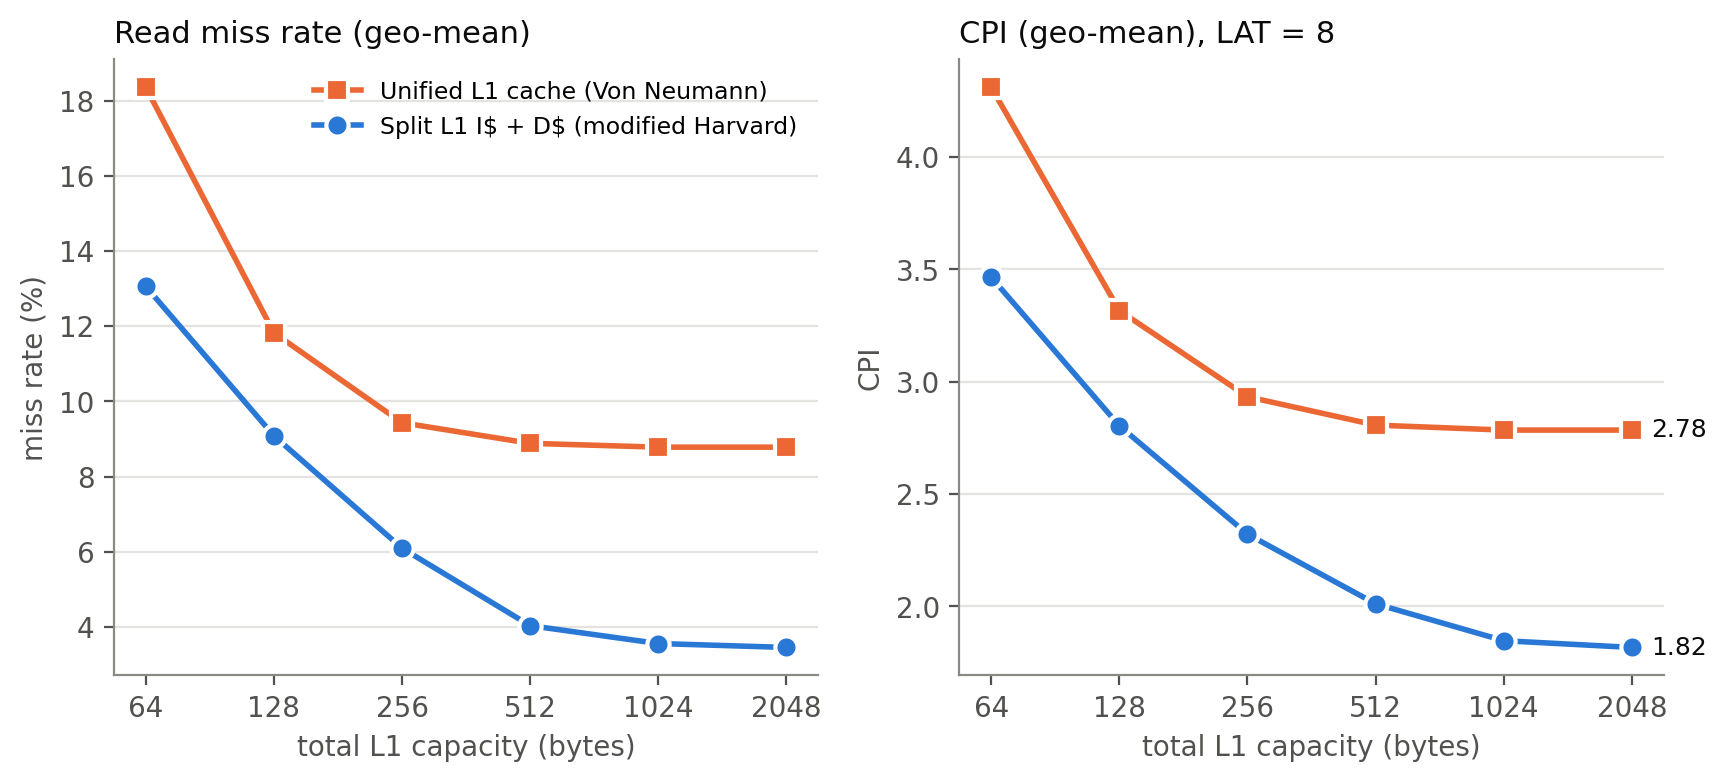
\includegraphics[width=\columnwidth]{l1_size_sweep.png}
\caption{Miss rate and CPI vs total L1 capacity ($\text{LAT}=8$, 16\,B lines).}
\label{fig:size}
\end{figure}

\begin{figure}[t]
\centering
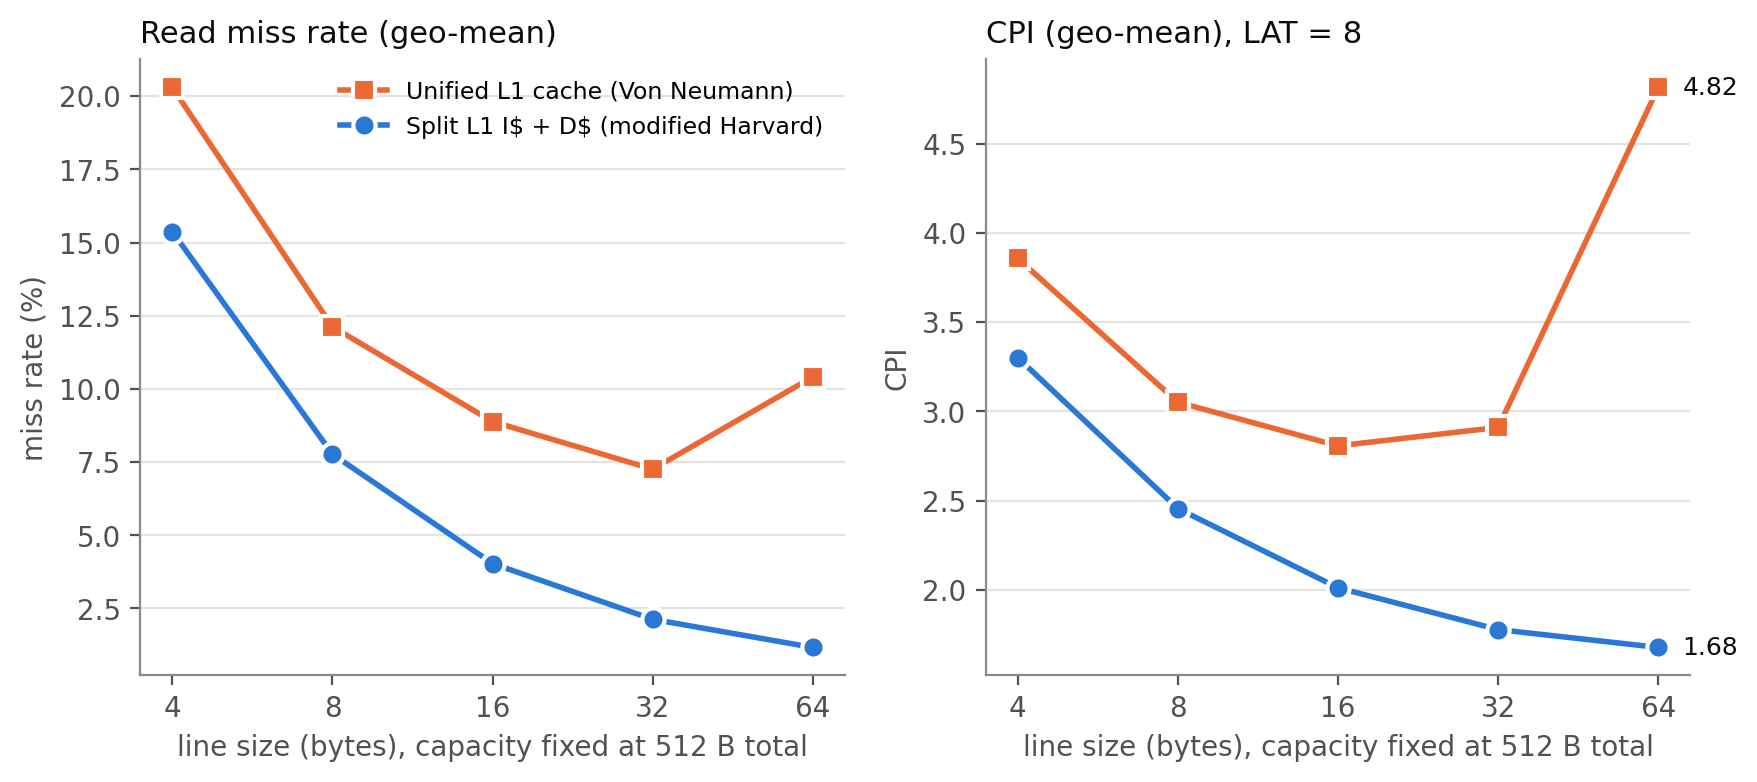
\includegraphics[width=\columnwidth]{line_size_sweep.png}
\caption{Miss rate and CPI vs line size (512\,B total, $\text{LAT}=8$).}
\label{fig:line}
\end{figure}

\subsection{Timing behaviour (waveform)}
Fig.~\ref{fig:wavehier} shows \texttt{vector\_add} on the split hierarchy at
$\text{LAT}=4$. A \texttt{lw} that misses holds the core for $\text{LAT}+W=8$
cycles while the D-line is refilled; afterwards the loop runs with no stalls.
Every \texttt{sw} completes in one cycle and its write to main memory
(``D write'') proceeds in the background while the following \texttt{addi},
\texttt{bne} and the next \texttt{lw} keep hitting in both caches. This is the
\emph{simultaneous access} the project asks us to analyse: instruction fetch,
data access and lower-level traffic all overlap.

\begin{figure*}[t]
\centering
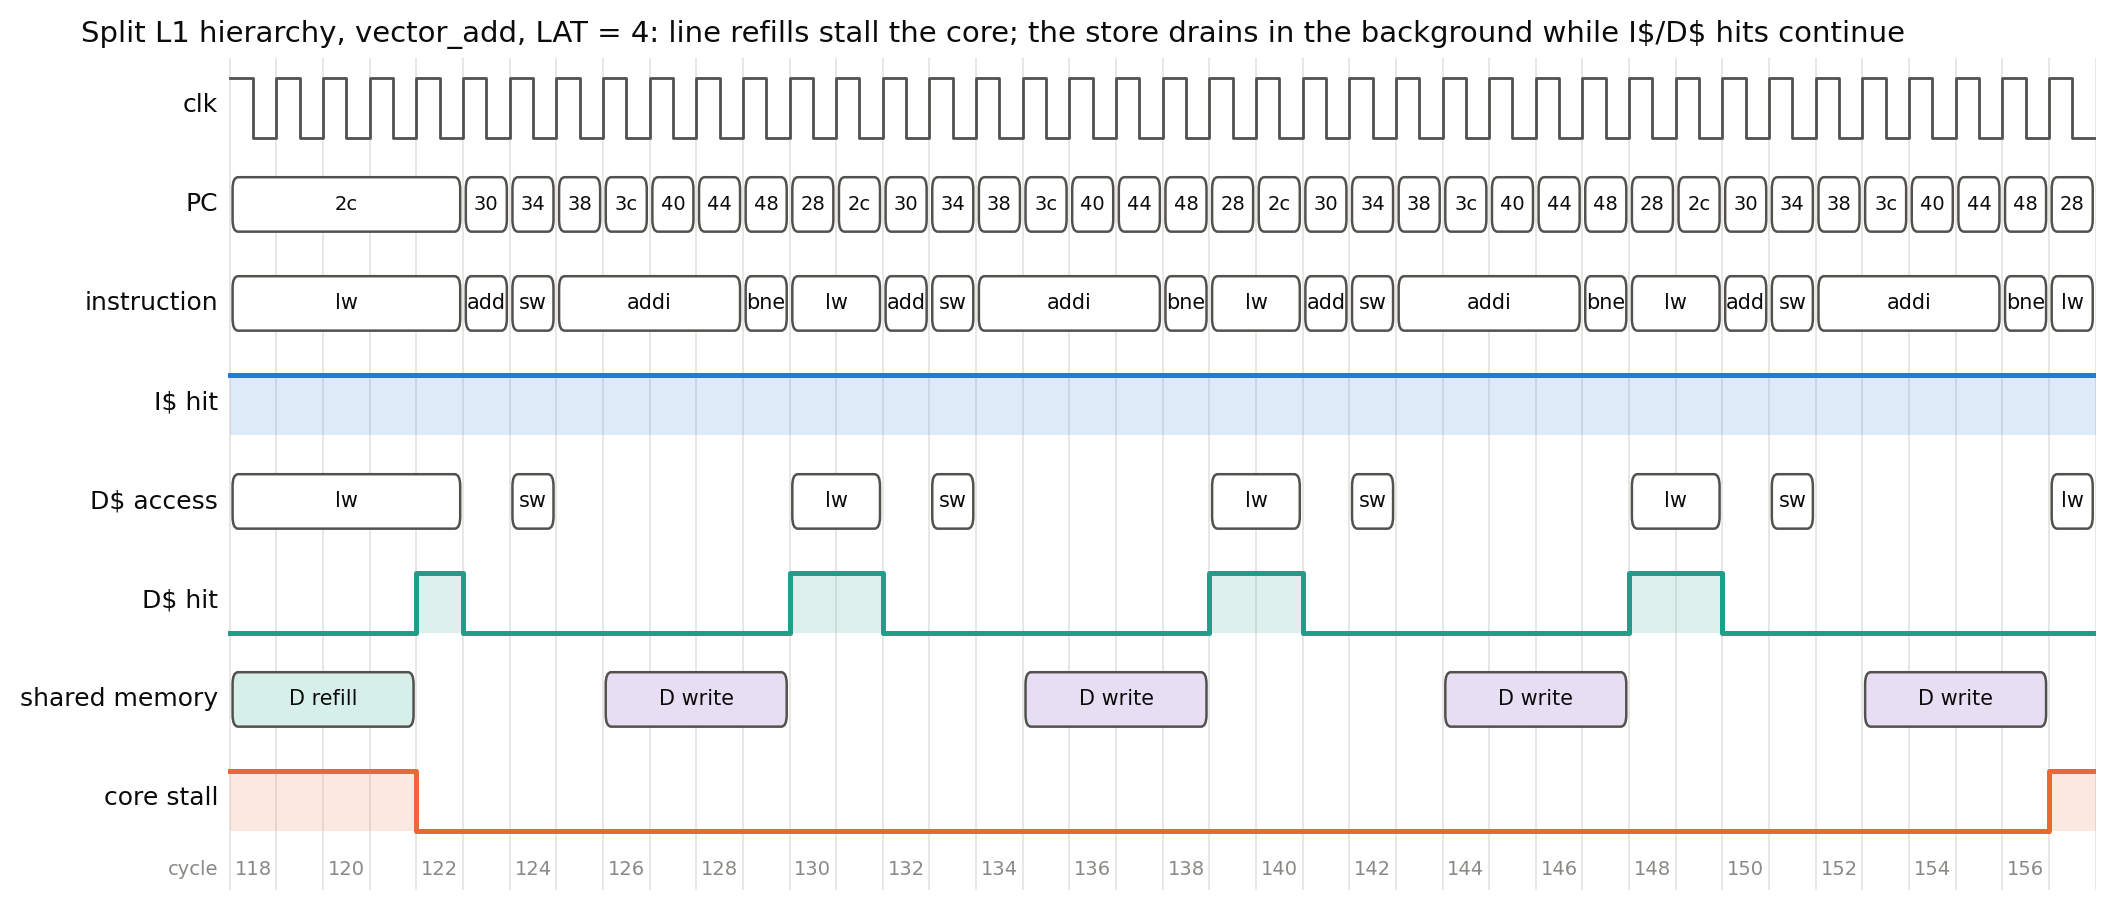
\includegraphics[width=0.85\textwidth]{wave_hierarchy.png}
\caption{Split-L1 hierarchy waveform (\texttt{vector\_add}, $\text{LAT}=4$):
a D-refill stalls the core, then store drains overlap with I/D hits.}
\label{fig:wavehier}
\end{figure*}

\subsection{Synthesis}
All top levels were synthesised with Yosys for a Xilinx 7-series target
(\texttt{synth\_xilinx}); Table~\ref{tab:synth} lists the results. The
performance counters drive no pins and are removed, so the numbers cover only
the core and memory system. A 256\,B cache costs 175 LUTs and 98 flip-flops
(tags, valid bits, write buffer, FSM). The split hierarchy uses about 5\,\%
\emph{fewer} LUTs than the unified one: two small caches need less
multiplexing than one port arbiter plus a cache twice the size. The
``path'' column is Yosys' longest combinational path between registers
(cells\,+\,nets, RAM cells cut). Without place-and-route it is only a
relative indicator, not an Fmax. It is larger for both single-port designs
because static analysis sees a (false) path through the shared port twice:
fetch $\rightarrow$ decode $\rightarrow$ ALU $\rightarrow$ data address
$\rightarrow$ the same memory.

\begin{table}[h]
\caption{Yosys synthesis (Xilinx 7-series primitives)}
\label{tab:synth}
\centering
\setlength{\tabcolsep}{4pt}
\begin{tabular}{lrrrr}
\toprule
Design & LUT & FF & LUTRAM & path \\
\midrule
Harvard (Phase I)            & 874   & 129 & 140 & 15 \\
Von Neumann (Phase I)        & 1\,210 & 162 & 268 & 78 \\
Split L1 hierarchy (proposed)& 1\,676 & 303 & 388 & 23 \\
Unified L1 hierarchy         & 1\,770 & 315 & 387 & 60 \\
One L1 cache, 256\,B         & 175   & 98  & 12  & 7 \\
\bottomrule
\end{tabular}
\end{table}

\subsection{Limitations}
The core is single-cycle, so an instruction's fetch and its data access
already happen in one cycle; a pipelined core would see an even larger
benefit from split paths. The caches are direct-mapped with a one-entry
write buffer, and the timing results come from simulation and
pre-place-and-route synthesis, not from hardware.

% ---------------------------------------------------------------------------
\section{Individual Contributions}
\begin{table}[h]
\caption{Contribution of each member}
\label{tab:contrib}
\centering
\renewcommand{\arraystretch}{1.15}
\begin{tabular}{p{0.2\columnwidth}p{0.72\columnwidth}}
\toprule
Member & Phase I / Phase II contribution \\
\midrule
Aaryan Yadav (2401010011) & \textbf{I:} core: \texttt{pc}, \texttt{regfile}, \texttt{alu}, \texttt{imm\_gen}, \texttt{control\_unit}, \texttt{cpu\_core}. \textbf{II:} core stall interface (\texttt{d\_wreq}), integration of \texttt{modharvard\_top.v}, Yosys synthesis flow (\texttt{synth/}). \\
Shashwat Sinha (2401010438) & \textbf{I:} \texttt{imem.v}, assembler + golden ISS, four test programs. \textbf{II:} ISS access trace, golden cache model (\texttt{cache\_model.py}), new benchmarks \texttt{matmul}, \texttt{memcpy}, \texttt{unrolled\_sum}. \\
Shivam Mishra (2401010442) & \textbf{I:} \texttt{dmem}, \texttt{addr\_decoder}, \texttt{rw\_control}, \texttt{io\_regs}, \texttt{harvard\_top}. \textbf{II:} \texttt{l1\_cache.v} (I/D/unified cache, write buffer, LUT-RAM mapping), uncached I/O fence. \\
Himank Kaushik (2401010187) & \textbf{I:} \texttt{unified\_mem}, VN arbiter, \texttt{perf\_counters}. \textbf{II:} shared \texttt{main\_mem.v}, \texttt{mem\_arbiter.v}, \texttt{unicache\_top.v} baseline, \texttt{hier\_perf.v} counters, AMAT analysis. \\
Satyam Kumar (2401010429) & \textbf{I:} testbenches, regression, figures, report, video. \textbf{II:} \texttt{tb\_hier.v}, \texttt{tb\_l1\_cache.v}, sweep/regression \texttt{run\_hier.py}, Phase II figures, this report. \\
\bottomrule
\end{tabular}
\end{table}

% ---------------------------------------------------------------------------
\section{Conclusion}
We implemented and verified a Harvard memory organisation (program counter,
instruction memory, data memory, address decoder, read/write control, I/O) and
extended it with a shared lower-level memory into a modified-Harvard
hierarchy. Each design was compared with a shared-memory counterpart built from
identical core RTL. With ideal memories, separate instruction and data paths
remove the structural hazard and run at CPI\,=\,1 instead of
$1+f_{\text{mem}}$. With a slow shared memory, splitting the paths alone helps
little (2--8\,\%), because the bottleneck moves to the shared memory. Split L1
caches restore the benefit: I- and D-hits proceed in the same cycle, code and
data stop evicting each other, and the shared memory sees almost no
simultaneous requests. At $\text{LAT}=8$ the split hierarchy is $1.40\times$
faster than a unified cache of the same size and $6.1\times$ faster than no
cache, at about 5\,\% lower LUT cost. The unified cache's only advantage,
flexible capacity, appears only when one stream (here the code) outgrows its
half. Natural next steps are a pipelined core, set-associative caches, a deeper
write buffer and place-and-route timing on an FPGA board.

% ---------------------------------------------------------------------------
\section*{Repository}
All RTL, testbenches, programs, scripts, results (\texttt{docs/results.csv},
\texttt{docs/results\_hier.csv}, \texttt{docs/synth.csv}) and figures are in
the project GitHub repository; \texttt{sim/run\_all.sh} reproduces every
result in this report.

\begin{thebibliography}{00}
\bibitem{mca_projects} Rishihood University, ``Modern Computer Architecture: Projects 1--12, Architecture-oriented RTL projects,'' Course document, B.Tech (CS\&AI), 2026.
\bibitem{vonneumann1945} J. von Neumann, ``First draft of a report on the EDVAC,'' Moore School of Electrical Engineering, Univ. of Pennsylvania, 1945.
\bibitem{aiken1946} H. H. Aiken and G. M. Hopper, ``The automatic sequence controlled calculator,'' \textit{Electrical Engineering}, vol.~65, 1946.
\bibitem{backus1978} J. Backus, ``Can programming be liberated from the von Neumann style? A functional style and its algebra of programs,'' \textit{Commun. ACM}, vol.~21, no.~8, pp.~613--641, 1978.
\bibitem{wulf1995} W. A. Wulf and S. A. McKee, ``Hitting the memory wall: Implications of the obvious,'' \textit{ACM SIGARCH Comput. Archit. News}, vol.~23, no.~1, pp.~20--24, 1995.
\bibitem{smith1982} A. J. Smith, ``Cache memories,'' \textit{ACM Comput. Surv.}, vol.~14, no.~3, pp.~473--530, 1982.
\bibitem{hill1989} M. D. Hill and A. J. Smith, ``Evaluating associativity in CPU caches,'' \textit{IEEE Trans. Comput.}, vol.~38, no.~12, pp.~1612--1630, 1989.
\bibitem{jouppi1993} N. P. Jouppi, ``Cache write policies and performance,'' in \textit{Proc. 20th Annu. Int. Symp. Computer Architecture (ISCA)}, 1993, pp.~191--201.
\bibitem{patterson2020} D. A. Patterson and J. L. Hennessy, \textit{Computer Organization and Design RISC-V Edition: The Hardware/Software Interface}, 2nd~ed. Cambridge, MA, USA: Morgan Kaufmann, 2020.
\bibitem{hennessy2017} J. L. Hennessy and D. A. Patterson, \textit{Computer Architecture: A Quantitative Approach}, 6th~ed. Cambridge, MA, USA: Morgan Kaufmann, 2017.
\bibitem{harris2021} S. L. Harris and D. M. Harris, \textit{Digital Design and Computer Architecture: RISC-V Edition}. Morgan Kaufmann, 2021.
\bibitem{riscv_isa} A. Waterman and K. Asanovi\'{c}, Eds., \textit{The RISC-V Instruction Set Manual, Volume I: Unprivileged ISA}, Document Version 20191213, RISC-V Foundation, 2019.
\bibitem{arm_m3} ARM Ltd., \textit{Cortex-M3 Technical Reference Manual}, ARM DDI 0337, 2010.
\bibitem{picorv32} C. Wolf, ``PicoRV32 -- A size-optimized RISC-V CPU,'' GitHub repository. [Online]. Available: \url{https://github.com/YosysHQ/picorv32}
\bibitem{icarus} S. Williams, ``Icarus Verilog.'' [Online]. Available: \url{https://steveicarus.github.io/iverilog/}
\bibitem{yosys} C. Wolf, ``Yosys Open SYnthesis Suite.'' [Online]. Available: \url{https://yosyshq.net/yosys/}
\end{thebibliography}

\end{document}
